\section{Thiết kế prompt để xây dựng cơ sở dữ liệu đồ thị và hệ thống đề xuất lộ trình học cho từng khóa học}

Trong hệ thống học tập này, LLM (Language Model) được sử dụng để hỗ trợ việc trích xuất thông tin về người học và tài nguyên học tập, từ đó giúp đề xuất các tài nguyên học tập phù hợp với mục tiêu học tập của người dùng. Quy trình này được thực hiện thông qua một chuỗi các bước được mô tả chi tiết dưới đây.
\section{Thiết kế prompt để xây dựng đồ thị tri thức từ nguồn học liệu (bài giảng, module,...)}
Việc xây dựng đồ thị từ nguồn học liệu sẽ được thực hiện bởi mô hình ngôn ngữ lớn, và dữ liệu sẽ được thêm vào cơ sở dữ liệu đồ thị bằng kỹ thuật \emph{function calling}:

Context: You are an assistant helping teachers and instructors process their learning resources.

Your role is to analyze and extract data from various learning materials (such as courses, lessons, 
learning modules, assignments, exercises, etc.) and convert it into a format suitable for 
insertion into a graph database. This database will support a personalized learning resource 
recommendation system tailored for students.

Your main task is to use the tool `AddLearningResource` to categorize each learning resource 
and identify relevant concepts. For each learning resource, you must identify and list at least 
5 related concepts that represent the key ideas or topics covered.
    
Instructions:
\begin{enumerate}
    \item Carefully examine the provided JSON data and understand the main topics of the resource.
    \item Use `add\_learning\_resource` to log the resource details and associated concepts.
    \item Ensure each resource has at least 5 related concepts to maximize the utility of the recommendation system.
    \item If the input data is a JSON array, please call AddLearningResource function for each learning
resource in the array.
Output your findings in a structured format.
\end{enumerate}
Câu prompt trên sử dụng function calling để mô hình có thể tự động thực hiện các tác vụ sau khi phân tích tài nguyên học tập, trong đó:
\begin{itemize}
    \item  Mô hình nhận diện các khái niệm chính từ nội dung của tài liệu học tập, chẳng hạn như "Networking", "Machine Learning", và các chủ đề liên quan. Các khái niệm này giúp xây dựng một cấu trúc đồ thị tri thức, từ đó hỗ trợ hệ thống gợi ý tài nguyên học tập cá nhân hóa cho người học.
    \item Sau khi trích xuất các khái niệm, mô hình sử dụng hàm \texttt{AddLearningResource} để ghi tài nguyên và các khái niệm vào cơ sở dữ liệu đồ thị. Mỗi tài nguyên học tập được gắn với các thuộc tính như độ khó (difficulty) và độ liên quan (relevance), giúp phân loại tài nguyên học tập theo các tiêu chí quan trọng.
\end{itemize}

\subsection{Cấu Trúc Đồ Thị}
Hệ thống sử dụng cơ sở dữ liệu đồ thị Neo4j để lưu trữ và quản lý các khái niệm học tập, tài nguyên học tập, và mối quan hệ giữa chúng. Cấu trúc đồ thị bao gồm các loại node và mối quan hệ sau:

\begin{itemize}
    \item \textbf{Concept:} Mỗi node đại diện cho một khái niệm học tập.
    \item \textbf{Learning Resource:} Các node tài nguyên học tập đại diện cho các bài giảng, sách, video, tài liệu học tập, ví dụ: "Video bài giảng về phương trình bậc hai", "Bài viết về đạo hàm".
    \item \textbf{Learner:} Node người học chứa thông tin về người học, bao gồm các khái niệm mà họ đang học và mức độ thành thạo đối với các khái niệm này.
\end{itemize}

Các mối quan hệ giữa các node bao gồm:
\begin{itemize}
    \item \textbf{COVERS:} Quan hệ giữa tài nguyên học tập và khái niệm mà tài nguyên đó đề cập đến. Mối quan hệ này có thuộc tính \textbf{difficulty}, đại diện cho độ khó của tài nguyên học tập đối với khái niệm đó. Ví dụ: Một video có thể "COVERS" khái niệm "Phương trình bậc hai" với độ khó là 0.8.
    \item \textbf{LEARNS:} Quan hệ giữa người học và khái niệm mà họ đang học. Mối quan hệ này có thuộc tính \textbf{proficiency}, biểu thị mức độ thành thạo của người học đối với khái niệm đó. Ví dụ: Người học "LEARNS" khái niệm "Lập trình Python" với mức độ thành thạo là 0.6.
\end{itemize}

\subsection{Thiết kế prompt cho việc đề xuất lộ trình học}
Việc đánh giá các tài nguyên học tập phù hợp sẽ được phụ trách bởi LLM. Sau đây là câu prompt đầu vào của hệ thống:

\begin{verbatim}
    You are a teacher assistant, and your task is to recommend learning 
    resources based on the learner’s profile. Here’s how the process works:

    Receive the learning goal from the learner.

    Invoke the function get_learner_profile_and_learning_resources with
    the list of analyzed concepts. This will return two things:
        The learner’s profile, which contains the proficiency level
        (0 to 1) for each concept. For instance:
            High proficiency (0.8-1): The learner is very skilled in 
            the concept (e.g., Linked List).
            Low proficiency (0.0-0.3): The learner is not familiar with 
            the concept (e.g., Binary Tree).
            Medium proficiency (0.3-0.7): The learner has some experience
            but needs improvement (e.g., sorting algorithms).
        A list of learning resources that match the learner’s needs.

    Select the top 5 most suitable resources, based on the learner's 
    profile and the resources returned.
        For each resource, explain why it is a good match for the learner:
            Focus on what the learner needs to improve on and how the 
            resource addresses those weaknesses.
            Avoid mentioning numerical proficiency, but instead focus on
            the learner’s needs.
            Explain what the learner can achieve by interacting with 
            each resource.

    Call the lp_recommender_response tool with your analysis and 
    recommendations.

   Example:

    Learning Goal: Mastering Binary Trees

        Learner Profile:
            Binary Trees: Proficiency = 0.3 (moderate skill)
            Data Structures: Proficiency = 0.8 (high skill)
            Algorithms: Proficiency = 0.5 (moderate skill)

        Learning Resources:
            Resource 1: "Binary Tree Fundamentals" (difficulty 0.4)
            Resource 2: "Advanced Binary Tree Algorithms" (difficulty 0.7)
            Resource 3: "Data Structure Optimization" (difficulty 0.6)
            Resource 4: "Understanding Tree Traversals" (difficulty 0.5)
            Resource 5: "Recursive Tree Operations" (difficulty 0.6)

        Recommended Resources and Explanations:

            Resource 1: "Binary Tree Fundamentals"
            Based on your profile, you have a moderate understanding of
            Binary Trees, but there are still fundamental areas where
            you could improve. This resource will help you strengthen
            your foundational knowledge, ensuring that you grasp basic
            concepts and terminology. This is particularly important
            because a strong foundation in Binary Trees will make 
            advanced topics easier to comprehend.

            Resource 2: "Advanced Binary Tree Algorithms"
            Your current proficiency in Binary Trees shows you have a basic
            understanding, but there are gaps when it comes to more complex
            algorithms. This resource will help you expand your knowledge 
            of how Binary Trees can be manipulated and optimized through 
            more advanced techniques, which will enhance your overall 
            problem-solving ability.

            Resource 3: "Data Structure Optimization"
            Since you are already proficient in data structures, this resource
            will help you learn how to make data structures, including Binary
            Trees, more efficient. Understanding optimization strategies will
            not only improve your technical skills but will also help you 
            think more critically about performance in algorithms.

            Resource 4: "Understanding Tree Traversals"
            Although you have a moderate proficiency with Binary Trees, your
            understanding of traversal techniques may need refinement. This
            resource is designed to help you understand different tree traversal
            methods, which are crucial for manipulating and accessing data
            within Binary Trees. Mastering this concept will be vital for
            solving problems efficiently.

            Resource 5: "Recursive Tree Operations"
            Your profile suggests that you may not be fully comfortable with 
            recursive algorithms, which are essential for operations in Binary
            Trees. This resource will walk you through recursive techniques 
            and give you the confidence to handle recursive solutions within
            tree structures.
\end{verbatim}
Quy trình xử lý mục tiêu học tập và đề xuất tài nguyên học tập được thực hiện thông qua các bước sau:
\begin{enumerate}
    \item LLM sẽ sử dụng function calling để gọi các hàm trong hệ thống nhằm trích xuất các thông tin sau:
    \begin{itemize}
        \item Tất cả các khái niệm liên quan mà khóa học đó có đề cập sẽ được trích xuất.
        \item Từ các khái niệm trên, profile của người học sẽ được mô hình thành một vector nhiều chiều, trong đó, mỗi thành phần của một vector là mức độ thông thạo của người học ứng với một khái niệm nhất định.
        \item Tương tự với profile của người học, các tài nguyên học tập cũng sẽ được mô hình thành các vector, trong đó, mỗi một thành phần biểu diễn độ khó của tài nguyên đó với một khái niệm nhất định.
        \item Từ vector biểu diễn profile của người học và vector biểu diễn các tài nguyên học tập, độ phù hợp của người học ứng với một tài nguyên học tập tương ứng sẽ được tính bằng khoảng cách Euclid. Công thức tính Euclidean distance là:
    $$
    \text{Euclidean Distance} = \sqrt{\sum_{i=1}^{n} (x_i - y_i)^2}
    $$
    Trong đó, $x_i$ và $y_i$ là các component của vector $X$ và $Y$ tương ứng, đại diện cho các khái niệm hoặc tài nguyên học tập.
    \end{itemize}

    \item Sau khi có được profile của người học, các tài nguyên học tập tương ứng cũng như độ phù hợp, LLM sẽ phân tích, đánh giá để chọn ra cũng như giải thích chi tiết về cách mỗi tài nguyên giúp người học cải thiện khả năng thành thạo các khái niệm cần thiết. LLM sẽ trả về các giải thích dạng tự nhiên cho người học.
\end{enumerate}

\begin{figure}[h!]
    \centering
    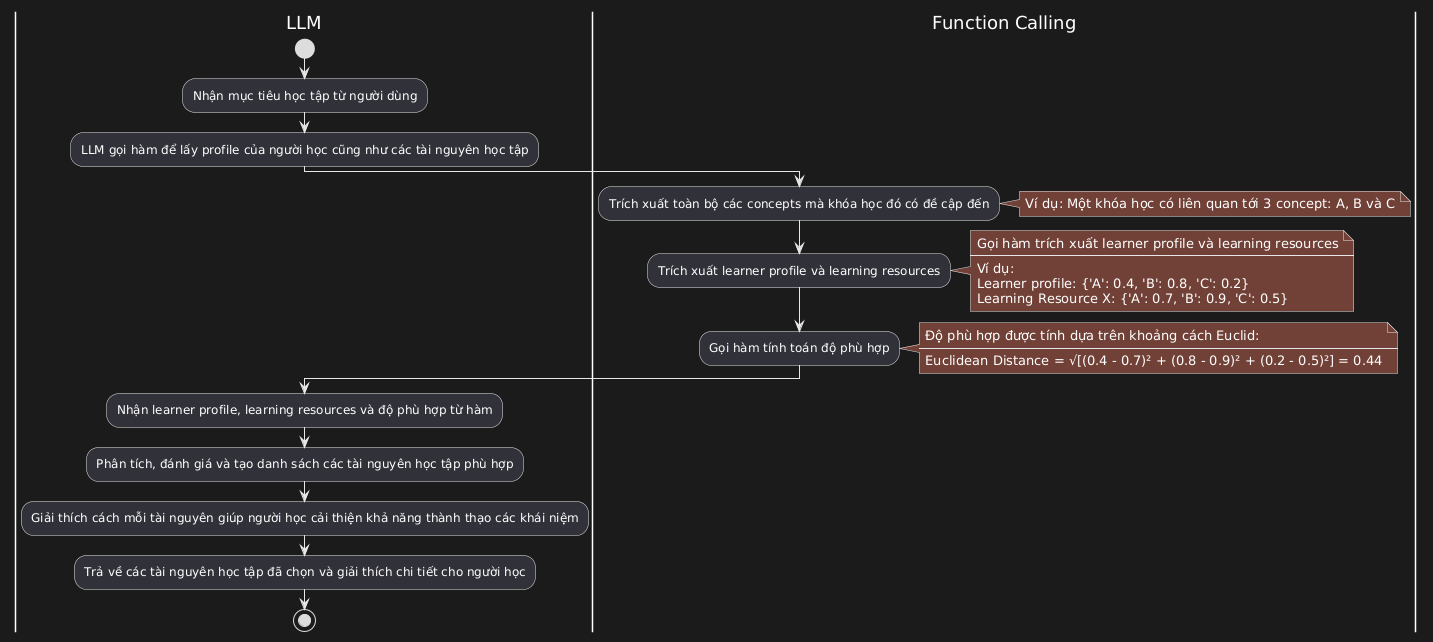
\includegraphics[width=\linewidth]{Images/flowchart-diagram.png}
    \caption{Giải thích chi tiết về các tài nguyên học tập}
    \label{fig:giaithuat}
\end{figure}

